\section{Case Study}
  \label{sec:case_study}
  \subsection{VPIC}
  In the section, we provide case study on BEE when running real HPC applications. We choose to test Vector Particle-In-Cell(VPIC) simulation tool \cite{bowers20080, bowers2008ultrahigh, bowers2009advances} on BEE. VPIC is a general purpose particle-in-cell simulation tool for modeling kinetic plasmas in multiple spatial dimensions. VPIC is large scale parallel application that runs on multiple nodes using MPI and pthreads. It has optimzied for modern computing architectures by using short-vector, single-instruction-multiple-data (SIMD) instructions and cache optimization. Before the simulation begin, VPIC first need to load input deck and user configuration from files and write to output when done. Flexible checkpoint-restart semantics enabling VPIC checkpoint files to be read as input for subsequent simulations. VPIC has a native I/O format that interfaces with the high-performance visualization software Ensight and Paraview. 

We evaluate the performance of VPIC on our BEE framework on HPC systems and cloud computing system with  its performance on bare metal HPC system. For the HPC system, we choose to use our testbed cluster system - Darwin. It has 16 Galton nodes, which have KVM enabled. Each node has two 8-core Intel Ivy Bridge E5-2650 v2 CPUs with 251GB RAM. For the cloud computing system, we choose to use Amazon Web Service. In order to get similar performance, we choose to use c3.4xlarge for each node on the cluster we deployed on AWS. Each node is equipped with Intel Xeon E5-2680 v2 CPUs with 16 vCPU cores and 30GB RAM. 


\begin{figure}[h]
    \centering
    \caption{VPIC scale up test on BEE and HPC host}
    \label{vpic-test}
    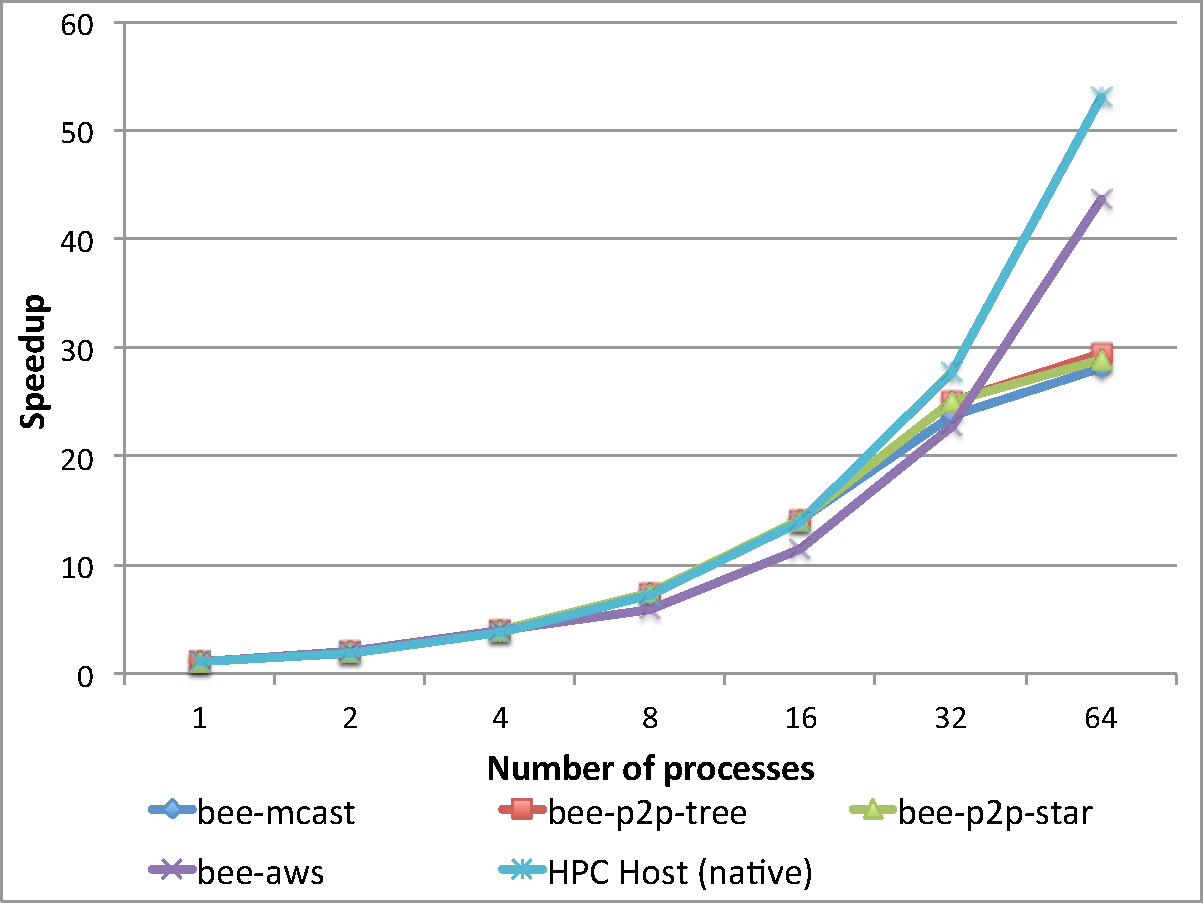
\includegraphics[width=0.5\textwidth]{figures/vpic-test.pdf}
\end{figure}

We test VPIC on different environment from using 1 process to 256 processes, which ranges from 1 computing node to 16 computing nodes. As shown in \textbf{Figure \ref{vpic-test}}, BEE-AWS solution scales similar to native host.  
